\chapter{Introduction}\label{chap:intro}
\textit{While the majority of this chapter was written for the thesis, parts of Sec \ref{sec:astero_intro} were written for \cite{2017North} and have been adapted from the introduction in that work to limit repetition. \textbf{YOU WANT SOMETHING LIKE THIS AT THE START OF EACH SCIENCE CHAPTER TOO, TO SHOW WHAT YOU DID AND ANY ACKNOWLEDGEMENTS OF OTHER PEOPLE}}

\section{Introduction}
... 

In this thesis we ...

Before we start on the main body of the thesis, the contents of each chapter and the main themes within are given in outline first.

Chapter ...

Chapter ...

Chapter ...

In Chapter ...

In Chapter ...
Finally the thesis is concluded in Chapter ...


\section{Space Weather}\label{sec:intro_SW}
\subsection{Forbush Decreases}\label{sec:intro_FDs}
...
\subsection{Ground Level Enhancements}\label{sec:intro_GLEs}
...


\section{Cosmic Rays}\label{sec:intro_CRs}
\subsection{...}
...

\section{The HiSPARC Experiment}\label{sec:intro_HiSPARC}
\subsection{HiSPARC Project}

HiSPARC stands for \textit{\textbf{Hi}gh \textbf{S}chool \textbf{P}roject on \textbf{A}strophysics and \textbf{R}esearch with \textbf{C}osmics}, and it is a scientific outreach project that was initiated in the Netherlands in 2002 \citep{bartels_hisparc_2012}. The HiSPARC project has two main goals: the study of \gls{uhecr} for astroparticle physics research, and to serve as a resource to expose high school students to scientific research \citep{bartels_hisparc_2012}.

HiSPARC is a global network of muon detectors spread across the Netherlands, Denmark, the UK, and Namibia. The detectors at each station record muon counts and may be used for many scientific experiments, such as: reconstruction of the direction of a cosmic ray induced air shower, reconstruction of the energy of the air shower's primary particle, investigation between the atmospheric conditions and the number of cosmics rays observed, etc.

Data recorded by the HiSPARC stations are stored and are available publicly at \url{http://www.hisparc.nl}, where the \gls{cr} counts, atmospheric data, station metadata, and more can be found.

%%%%%%%%%%%%%%%%%%%%%%%%%%%%%%%%%%%%%%%%%%%%%%%%%%%%%%%%%%%%%%%%%%%%%
\subsection{HiSPARC Detector and Station Configuration}

The detection philosophy of HiSPARC is to sample the footprints of \glspl{eas} using coincident triggers between scintillation detectors. As HiSPARC was set up as an outreach programme for high schools, this impacted detector design. Resources are limited in schools and the detectors are usually financed by the participating high schools, colleges, and universities. In addition, students (accompanied by their teachers and local node support staff) are responsible for assembly and installation their detectors, which are typically installed on the roofs of schools. Due to this, the detectors needed to be cheap, robust, and easily maintainable, therefore the scintillation detector was selected for the HiSPARC network.

Scintillators consist of materials that emit light when charged particles pass through them with sufficient energy to ionise the scintillator material. The total light produced is proportional to the number of charged particles, and can be collected by a \gls{pmt}. Each HiSPARC detector utilises a plastic scintillator of dimensions 1000~mm x 500~mm x 20~mm, providing a detection area of 0.5~$\mathrm{m}^2$. A vertically incident \gls{mip} has a most probable energy loss in 2~cm of the scintillation material of 3.51~MeV ($\equiv 1$ \gls{mip}) \citep{van_dam_hisparc_2020}.

The scintillator is glued to a triangular/`fish-tailed' light-guide (dimensions, base: 500~mm; top: 25~mm; height: 675~mm), and a light-guide adapter provides the optical interface between the square end of the light-guide and the cylindrical aperture of the \gls{pmt}. The configuration of a single HiSPARC detector is shown in Figure~\ref{fig:HS_scintillator}. 

\begin{figure}[ht!]
	\centering
	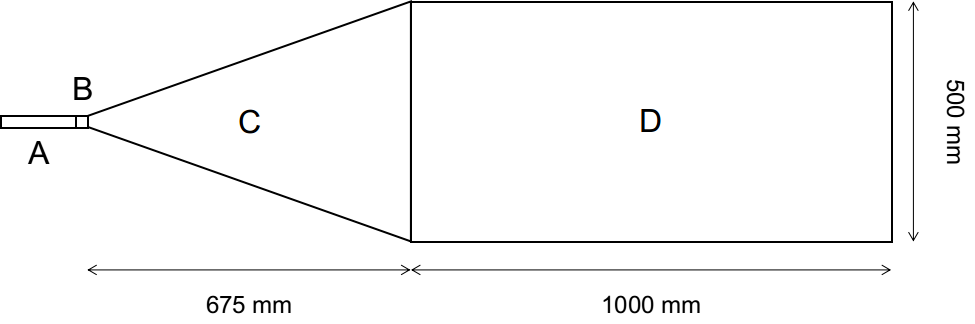
\includegraphics[width=0.75\columnwidth]{config.png}
	\caption{Schematic diagram of the HiSPARC scintillation detector. (A): PMT; (B): light-guide adaptor; (C): light-guide; (D): scintillator.}
	\label{fig:HS_scintillator}
\end{figure}

The scintillator is made of a material consisting of polyvinyltoluene as the base, with anthracene as the fluor, and the emission spectrum peaks at a wavelength of 425~nm \citep{fokkema_hisparc_2012, bartels_hisparc_2012}. The light-guide is made from \gls{pmma} and has a comparable refractive index to the scintillator (1.58 and 1.49, respectively), reducing refraction effects between the two materials \citep{van_dam_hisparc_2020}.

The \gls{pmt} used is an ETEnterprises 9125B \gls{pmt}, with a 25~mm aperture,  blue-green sensitive bialkali photocathode, and 11 high-gain dynodes \citep{bartels_hisparc_2012,et_enterprises_data_2020}. The quantum efficiency of the \gls{pmt} used in the HiSPARC detectors peaks at around 375 nm at 28\%, and at 425 nm the quantum efficiency is 25\% \citep{fokkema_hisparc_2012}. 

Each detector is wrapped in aluminium foil (thickness 30~$\mu$m) and a black, vinyl material (thickness 0.45~mm), which is usually used as a pond liner, to ensure light-tight detectors and to reduce the noise level from stray photons \citep{van_dam_hisparc_2020}. In addition, each detector is placed inside of its own a plastic roof box to again ensure that it is light-tight, and to also ensure that it is weather-proof, as the detectors are usually located on the roofs of schools, colleges, and universities.

A HiSPARC station combines either 2 or 4 detectors, to observe coincident muons (`events'), and typical configurations of each are shown in Figure~\ref{fig:HS_station_layouts}. The separation between detectors varies from station-to-station. In addition some stations have the capability to measure the local atmospheric properties, such as temperature, pressure, relative humidity etc. Moreover, some stations also record the `singles' rates, i.e. the frequency at which an individual detector is triggered, independently of the other detectors in the station. The singles rates are important when investigating non-\gls{eas} events.


\begin{figure}[ht!]
	\centering
	\subfloat[Two-detector station configuration]{
\includegraphics[width=0.6\columnwidth]{HS_2D2.png}} 
	\qquad
	\subfloat[Four-detector station configuration (triangle arrangement)]{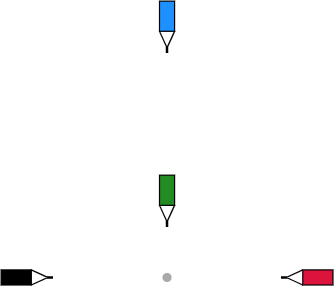
\includegraphics[width=0.6\columnwidth]{HS_4D_t2.png}}
	\qquad
	\subfloat[Four-detector station configuration (diamond arrangement)]{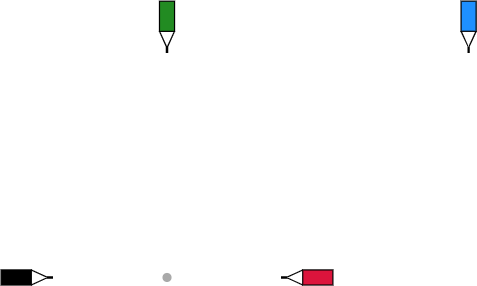
\includegraphics[width=0.6\columnwidth]{HS_4D_d2.png}}
	\caption{Typical formations of two-detector and four-detector stations. In each, the grey circle denotes a GPS antenna which is located in between the detectors to provide a precise timestamp for each signal.}
	\label{fig:HS_station_layouts}
\end{figure}


light pulse which is converted
into an electric pulse by the PMT. This pulse is
sampled and digitized at 400 MHz

The \glspl{pmt} of the detector in a station are connected to HiSPARC electronics boxes, which sample and digitise the signal at a rate of 400~MH, and each \glspl{pmt} is connected to the electronics box using cables of a standard length of 30~m, to minimise any timing offsets between detectors \citep{fokkema_hisparc_2012, van_dam_hisparc_2020}. The electronics boxes are capable of controlling and reading two \glspl{pmt}, therefore a four-detector station requires two electronics boxes: a master and a slave.

The HiSPARC experiment is set up in such a way as to ensure that each station across the HiSPARC network reads a similar count rate of muons, in order to aid the direct comparison between the different stations in the network. When configuring the station, a trigger threshold must be applied for the \gls{pmt} signals. This is standardised across the HiSPARC network and can be seen in relation to a detector trigger pulse in Figure~\ref{fig:HiSPARC_trace}. There are two thresholds, low: 30~mV, which represents 0.2 of a \gls{mip}; high: 70~mV, which represents 0.5 of a \gls{mip} \citep{fokkema_hisparc_2012, van_dam_hisparc_2020}. The thresholds were chosen to increase the sensitivity of the stations for observing gamma rays and low energy electrons, but this has the effect of making it more difficult to determine whether an individual detection is from a muon, or another \gls{mip}. This is why the HiSPARC network usually relies on detecting `events', from coincident muons.

Each detector in the network is set up such that the pulseheight spectrum peaks at a \gls{mpv} of $\sim 150$~mV (see Figure~\ref{fig:pulses}), and such that the high threshold allows a mean count rate on the order 100 counts per second and the low threshold allows a mean count rate of the order 400 counts per second; these can by tuned by adjusting the \gls{pmt} voltage. It could be argued that in setting up the detectors in this way, there is an immediate bias in the data to reject lower energy \glspl{cr}.

\begin{figure}[ht!]
	\centering
	\subfloat[Trigger pulse]{
		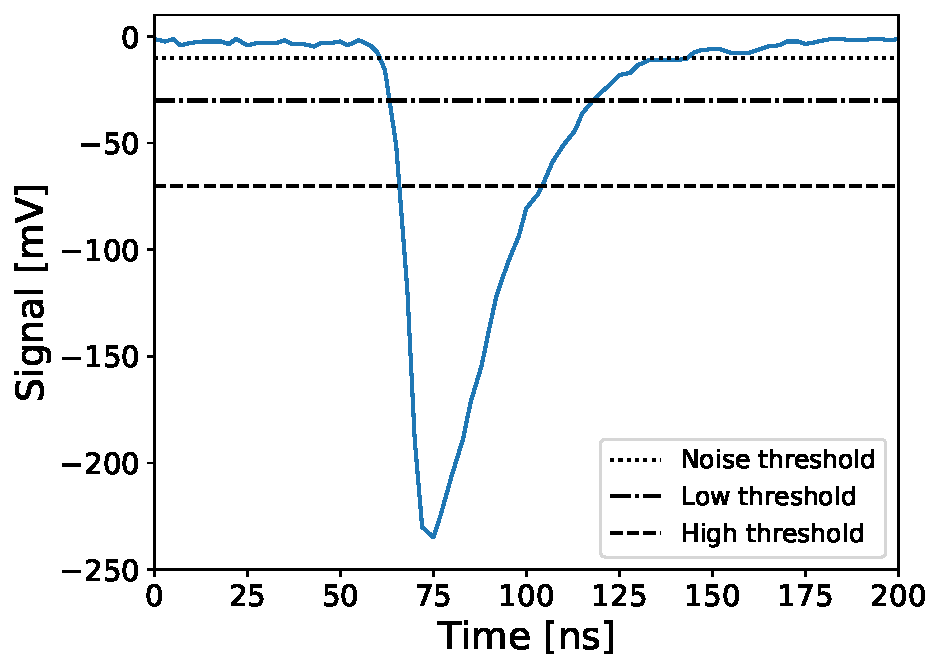
\includegraphics[width=0.48\columnwidth]{trace_plot.pdf}
		\label{fig:HiSPARC_trace}}
	%\qquad
	\subfloat[Pulseheight distribution]{
		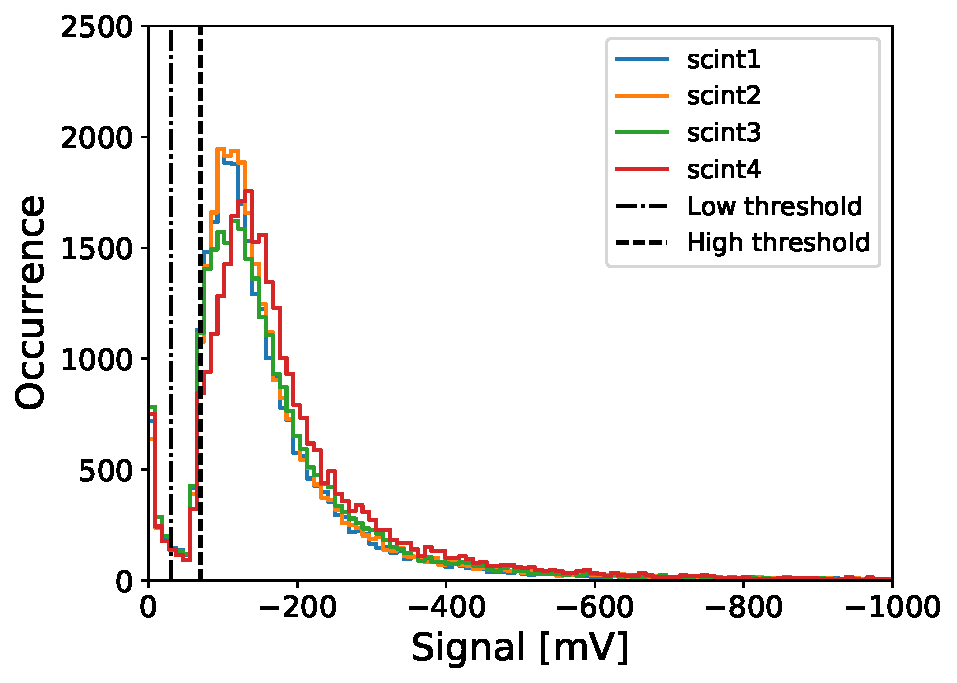
\includegraphics[width=0.48\columnwidth]{pulseheights.pdf}
		\label{fig:HiSPARC_pulseheight}}
	
	\caption{(a): An example PMT signal after digital conversion by the HiSPARC electronics box. The horizontal lines denote: the noise cut-off (dotted line), which is used for setting a limit when integrating the pulse height, to give the pulse integral; the low-voltage threshold (dash-dot); the high-voltage threshold (dashed). (b) The pulse height distribution over the course of a single day from HiSPARC station 501. The vertical lines show the low-voltage threshold (dash-dot) and the high-voltage threshold (dashed).}
	\label{fig:pulses}
\end{figure}

The pulse height spectrum (see Figure~\ref{fig:HiSPARC_pulseheight}) is composed of two main regions: the left side which falls off rather steeply and the main, asymmetric part of the spectrum which features a peak and a long tail. The left side of the spectrum is understood to be from high-energy photons (gamma rays) produced in air showers \citep{fokkema_hisparc_2012}. These high-energy photons may undergo pair production when interacting with the scintillator which may produce ionising electron and positron pairs. The trigger thresholds are placed to reject these noise signals from the data.

The main, asymmetric distribution which features a peak and a tail is from charged particles (muons and electrons) \citep{van_dam_hisparc_2020}. The mean energy loss of particles in a material is described by the Blethe-Bloch formula; however this does not account for fluctuations in energy loss \citep{fokkema_hisparc_2012}. A Landau distribution in fact describes the fluctuations in energy loss of particles. Due to the resolution of the HiSPARC detectors the distribution in Figure~\ref{fig:HiSPARC_pulseheight} is best described by the convolution of the Landau distribution with a normal distribution which describes the resolution of the detector \citep{fokkema_hisparc_2012}. The peak of the distribution, the most probable values (\gls{mpv}), is the most likely energy lost by a particle in the detector, i.e. the 3.51~MeV \gls{mip} \citep{van_dam_hisparc_2020}. It has been shown that the location of the \gls{mpv} can vary due to the effects of atmospheric temperature \citep{bartels_hisparc_2012, van_dam_hisparc_2020}.

The default trigger conditions for detecting an air shower event between multiple \glspl{pmt} within a station differ for a two/four-detector station. In a two-detector station, an event is recorded if the \gls{pmt} signals from both detectors exceed the low threshold within the coincidence time window ($1.5 \, \mu\mathrm{s}$). In a four-detector station, there are two conditions: (i) at least two detectors exceed the high threshold within the coincidence time window; (ii) at least three detectors exceed the low threshold within the coincidence time window. These are the default conditions, but there are other, user configurable ways of triggering the station.

The scientific goals that can be achieved also vary between the two/four-detector stations. When at least three detectors in a four-detector station observe particles of an \gls{eas}, the direction of the \gls{eas} (and thus the direction of the \gls{pcr}) can be acquired using triangulation calculations. When only two detectors in a station observe particles of an \gls{eas}, i.e. the limit for a two-detector station, it is only possible to reconstruct the arrival direction along the axis that connects the centres of those two detectors (thus it is not possible to reconstruct the direction of the \gls{pcr}).


\section{The Solar Mean Magnetic Field}\label{sec:intro_SMMF}
\subsection{...}
...


